\begin{frame}
  \frametitle{The DG method eases space (p-) adaptivity}
  \begin{columns}[t]
    \begin{column}{0.3\textwidth}
    \only<1>{
      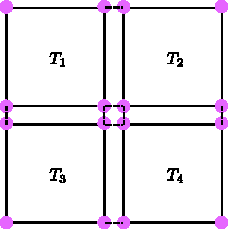
\includegraphics[width=1.0\textwidth]{pdf/box-mesh-after-split.pdf}
    }
    \only<2->{
      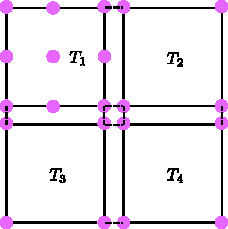
\includegraphics[width=1.0\textwidth]{pdf/box-mesh-after-split-p-refined.pdf}
    }
    \end{column}
    \begin{column}{0.7\textwidth}
      \only<1-2>{
    \def\svgwidth{1.0\textwidth}
    \import{pdf/}{lin-dg.pdf_tex}
  }
      \only<3->{
    \def\svgwidth{1.0\textwidth}
    \def\svgwidth{1.0\textwidth}
    \import{pdf/}{lin-dg-p-adapted.pdf_tex}
  }
    \end{column}
  \end{columns}
\end{frame}
%\begin{frame}
%  \frametitle{DG motivation}
%      \only<1>{
%    \def\svgwidth{1.0\textwidth}
%    \import{figures/trial-lecture/}{lin-dg.pdf_tex}
%  }
%      \only<2->{
%    \def\svgwidth{1.0\textwidth}
%    \def\svgwidth{1.0\textwidth}
%    \import{figures/trial-lecture/}{lin-dg-p-adapted.pdf_tex}
%  }
%\end{frame}
